% Ablations picture: two of the clearest ablations, drawn at 16 x 9 cm.
\documentclass[border=4pt]{standalone}
% Shared style for the poster's figures: the report's colours and box styles, in a sans font close to the
% template's Arial, sized for print on A1 (each figure is drawn at the size it has on the poster).
\usepackage[T1]{fontenc}
\usepackage{helvet}
\renewcommand{\familydefault}{\sfdefault}
\usepackage{xcolor}
\usepackage{tikz}
\usetikzlibrary{arrows.meta,positioning,fit,backgrounds,calc,shapes.geometric}
\usepackage{pgfplots}
\pgfplotsset{compat=1.18}
% numbers in the same sans font as the text, not the maths font
\pgfplotsset{/pgf/number format/assume math mode=true}
% no hyphenated words in the boxes
\hyphenpenalty=10000
\exhyphenpenalty=10000

\definecolor{modelfill}{HTML}{EDE9FE}
\definecolor{modelline}{HTML}{6D28D9}
\definecolor{codefill}{HTML}{F1F5F9}
\definecolor{codeline}{HTML}{475569}
\definecolor{solverfill}{HTML}{FEF3C7}
\definecolor{solverline}{HTML}{B45309}
\definecolor{peoplefill}{HTML}{EAF1F8}
\definecolor{peopleline}{HTML}{2E5C8A}
\definecolor{goodfill}{HTML}{E9F7EE}
\definecolor{goodline}{HTML}{2E8B57}
\definecolor{badfill}{HTML}{FDECEC}
\definecolor{badline}{HTML}{C0392B}
\definecolor{greyline}{HTML}{6B7280}
\definecolor{posterpurple}{HTML}{4B2A84}

\tikzset{
  bx/.style={draw, rounded corners=3pt, align=center, line width=1.2pt, inner sep=5pt, minimum height=11mm},
  mdl/.style={bx, draw=modelline, fill=modelfill},
  cde/.style={bx, draw=codeline, fill=codefill},
  slv/.style={bx, draw=solverline, fill=solverfill},
  ppl/.style={bx, draw=peopleline, fill=peoplefill},
  okb/.style={bx, draw=goodline, fill=goodfill},
  bad/.style={bx, draw=badline, fill=badfill},
  dec/.style={draw=codeline, fill=codefill, diamond, aspect=2.2, inner sep=2pt, align=center, line width=1.2pt},
  arr/.style={-{Stealth[length=4mm, width=3mm]}, draw=greyline, line width=1.6pt},
  darr/.style={arr, dashed},
  lb/.style={fill=white, inner sep=2pt}
}

\begin{document}
\fontsize{15}{18}\selectfont
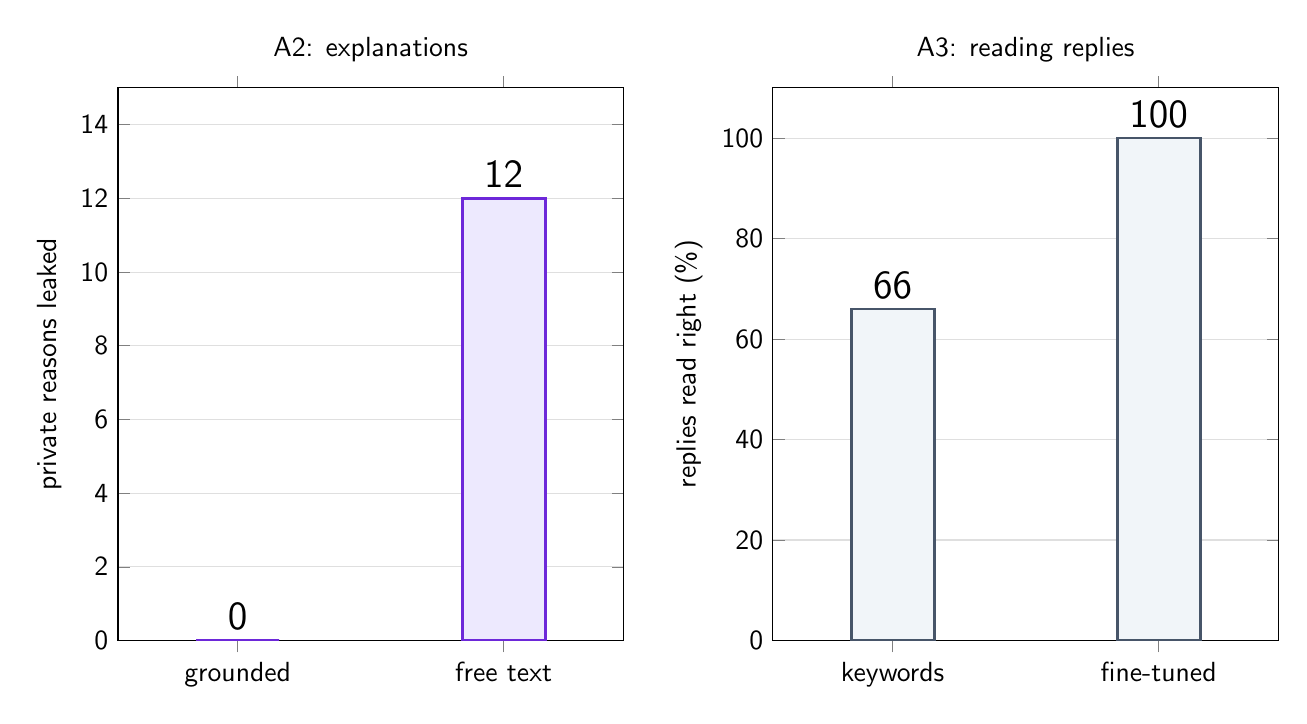
\begin{tikzpicture}
\begin{axis}[
  name=leaks, ybar, bar width=30pt, width=8cm, height=8.6cm,
  ymin=0, ymax=15, ylabel={private reasons leaked},
  symbolic x coords={grounded, free text}, xtick=data, enlarge x limits=0.45,
  title={A2: explanations}, ymajorgrids, grid style={gray!25},
  nodes near coords, every node near coord/.append style={font=\fontsize{14}{16}\selectfont}]
\addplot[fill=modelfill, draw=modelline, line width=1pt] coordinates {(grounded,0) (free text,12)};
\end{axis}
\begin{axis}[
  at={(leaks.east)}, anchor=west, xshift=1.9cm, ybar, bar width=30pt, width=8cm, height=8.6cm,
  ymin=0, ymax=110, ylabel={replies read right (\%)},
  symbolic x coords={keywords, fine-tuned}, xtick=data, enlarge x limits=0.45,
  title={A3: reading replies}, ymajorgrids, grid style={gray!25},
  nodes near coords, every node near coord/.append style={font=\fontsize{14}{16}\selectfont}]
\addplot[fill=codefill, draw=codeline, line width=1pt] coordinates {(keywords,66) (fine-tuned,100)};
\end{axis}
\end{tikzpicture}
\end{document}
